\documentclass[border=4pt]{standalone}
\usepackage{tikz}
\usetikzlibrary{arrows, positioning, shapes, fit}
\begin{document}
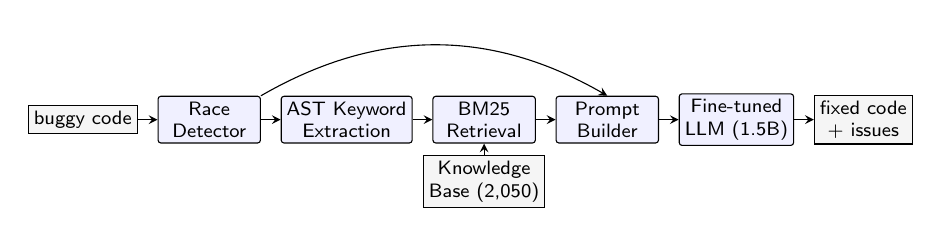
\begin{tikzpicture}[
  node distance=0.25cm and 0.25cm,
  box/.style={draw, rectangle, rounded corners=1pt,
              minimum width=1.3cm, minimum height=1.0em,
              font=\scriptsize\sffamily, align=center,
              inner sep=2pt, fill=blue!6},
  io/.style={draw, rectangle, rounded corners=0pt,
             minimum width=1.1cm, minimum height=1.0em,
             font=\scriptsize\sffamily, align=center,
             inner sep=2pt, fill=gray!8},
  arrow/.style={-stealth, thin},
]
  \node[io] (code) {buggy code};
  \node[box, right=of code] (det) {Race\\Detector};
  \draw[arrow] (code) -- (det);
  \node[box, right=of det] (ast) {AST Keyword\\Extraction};
  \draw[arrow] (det) -- (ast);
  \node[box, right=of ast] (bm25) {BM25\\Retrieval};
  \draw[arrow] (ast) -- (bm25);
  \node[io, below=0.15cm of bm25] (kb) {Knowledge\\Base (2,050)};
  \draw[arrow] (kb) -- (bm25);
  \node[box, right=of bm25] (prompt) {Prompt\\Builder};
  \draw[arrow] (bm25) -- (prompt);
  \draw[arrow] (det.north east) to[out=30, in=150] (prompt.north);
  \node[box, right=of prompt] (llm) {Fine-tuned\\LLM (1.5B)};
  \draw[arrow] (prompt) -- (llm);
  \node[io, right=of llm] (fix) {fixed code\\+ issues};
  \draw[arrow] (llm) -- (fix);
\end{tikzpicture}
\end{document}
